\documentclass{beamer}
\usepackage[utf8]{inputenc}
\usepackage[T1]{fontenc}

\title{Project Report}
\subtitle{\textit{Week 3}}
\date[]{2024/2025}
\author[Fritz]{Fritz Adelbertus Sitindaon}

\usetheme{Warsaw}
\setbeamertemplate{footline}[frame number]
% ===== Setup Font =====
\usepackage[sfdefault,lf]{carlito}
\usepackage[T1]{fontenc}
\renewcommand*\oldstylenums[1]{\carlitoOsF #1}

% ==== Import Math Packages =====
\usepackage{amsmath, amssymb, amsthm}
\usepackage{mathtools}

% ==== There required =====
\usepackage[dvipsnames]{xcolor}
\usepackage[most]{tcolorbox}
\def\wallpaper{wallpaper.jpg}

\def\R{\mathbb{R}}
\def\P{\mathbb{P}}
\def\N{\mathbb{N}}
\def\O{\mathbb{O}}


\def\nX{\mathcal{X}}
\def\nY{\mathcal{Y}}
\def\nT{\mathcal{T}}
\def\nU{\mathcal{U}}
\def\nB{\mathcal{B}}
\def\nS{\mathcal{S}}
\def\nP{\mathcal{P}}
\def\nA{\mathcal{A}}
\def\nF{\mathcal{F}}
\newcommand{\comp}[1]{\overline{#1}} 

\DeclarePairedDelimiter\abs{\lvert}{\rvert}
\DeclarePairedDelimiter\floor{\lfloor}{\rfloor}
\DeclarePairedDelimiter\cic{[ }{] }
\DeclarePairedDelimiter\oic{( }{] }
\DeclarePairedDelimiter\cio{[ }{) }
\DeclarePairedDelimiter\oio{( }{) }
\DeclarePairedDelimiter\set{\{ }{\} }
\DeclarePairedDelimiter\brk{(}{)}
\DeclarePairedDelimiter\seq{\langle}{\rangle}

\begin{document}

\begin{frame}
\titlepage
\end{frame}



\begin{frame}{Program Runs!}
    \begin{center}
        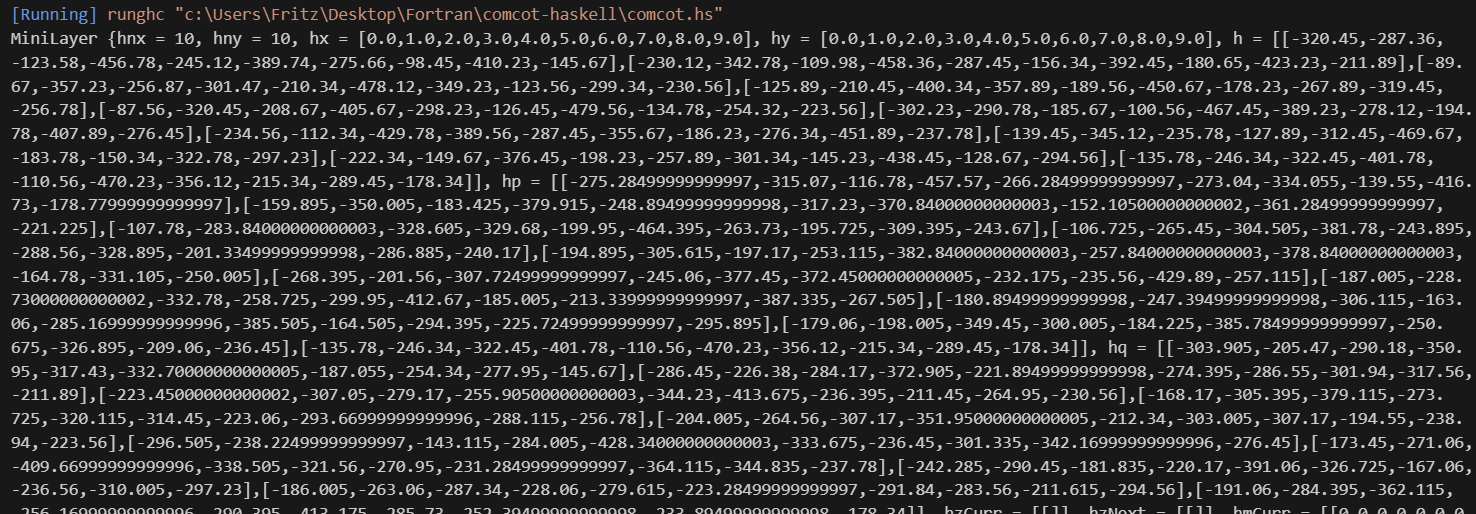
\includegraphics[scale=0.25]{figure/output.png}
    \end{center}
\end{frame}

\begin{frame}{Patterns}
    \begin{center}
        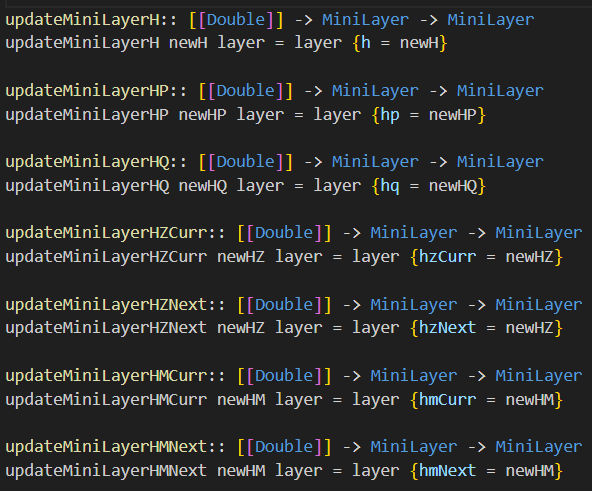
\includegraphics[scale=0.5]{figure/pattern1.png}
    \end{center}
\end{frame}

\begin{frame}{Patterns}
    \begin{center}
        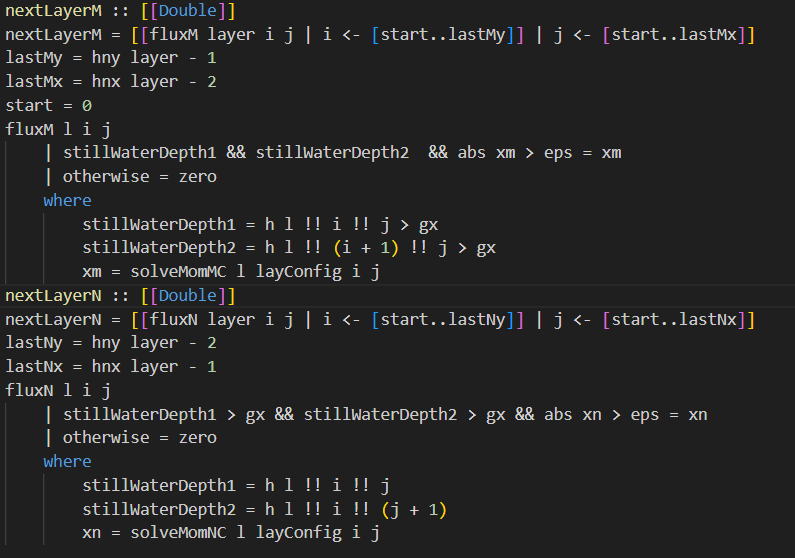
\includegraphics[scale=0.5]{figure/pattern2.png}
    \end{center}
\end{frame}

\begin{frame}{Patterns}
    \begin{center}
        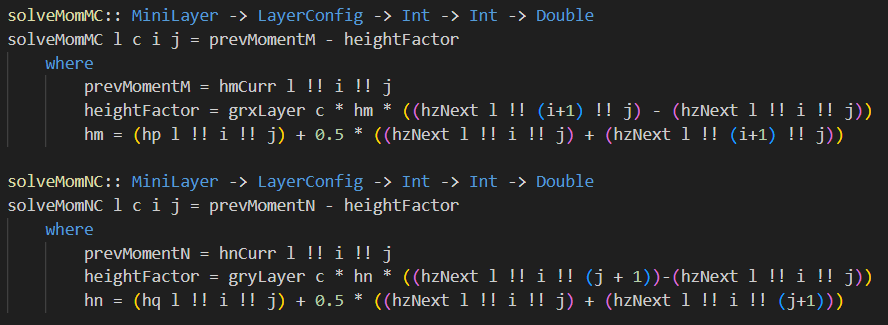
\includegraphics[scale=0.4]{figure/pattern3.png}
    \end{center}
\end{frame}

\begin{frame}{Patterns}
    \begin{center}
        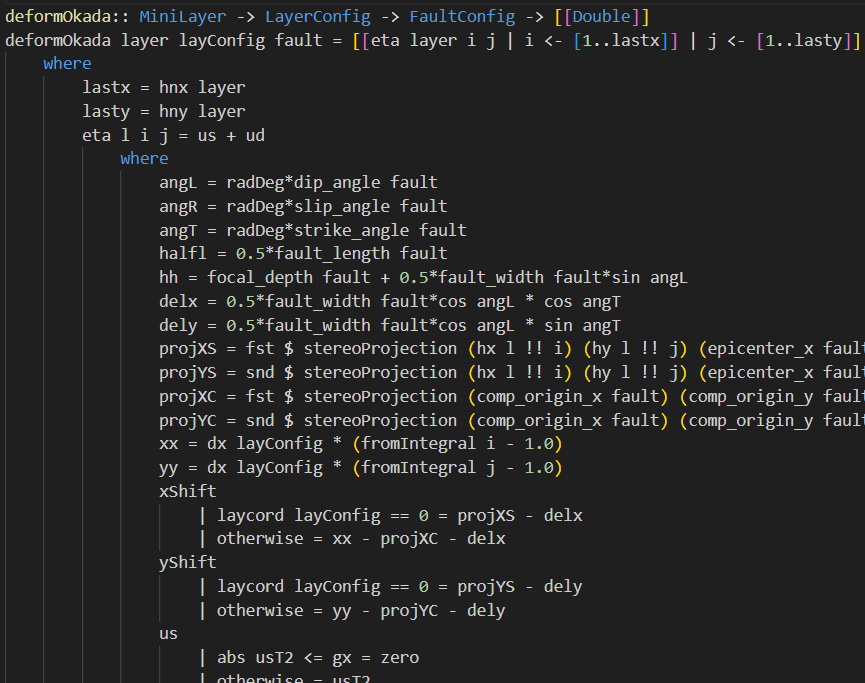
\includegraphics[scale=0.4]{figure/pattern4.png}
    \end{center}
\end{frame}

\begin{frame}{Patterns}
    \begin{center}
        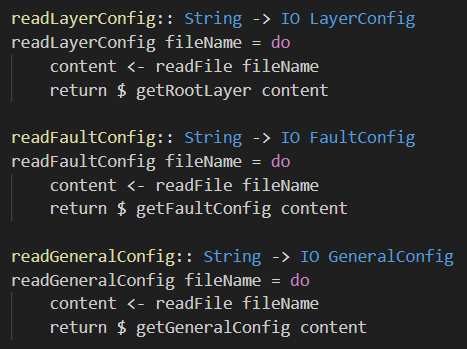
\includegraphics[scale=0.5]{figure/pattern5.png}
    \end{center}
\end{frame}

\begin{frame}{File Structure and Size}
    \begin{itemize}
        \item $type\_module.f90$: 180 lines
        \item $initialization.f90$: 2021 lines
        \item $all\_grids.f90$: 927 lines
        \item $boundaries.f90$: 439 lines
        \item $comcot.f90$: 526 lines
        \item $wavemaker.f90$: 362 lines
        \item $deform.f90$: 675 lines
        \item $landslide.f90$: 299 lines
        \item $mass.f90$: 205 lines
        \item $moment.f90$: 939 lines
        \item $dispersion.f90$: 1647 lines
        \item $hotstart.f90$: 138 lines
        \item $output.f90$: 1010 lines
    \end{itemize}
\end{frame}

\begin{frame}{Progress (compared to the original source code)}
    \begin{itemize}
        \item $type\_module.f90$: \textcolor{green}{60\%}
        \item $initialization.f90$: \textcolor{orange}{50\%}
        \item $all\_grids.f90$: \textcolor{red}{0\%}
        \item $boundaries.f90$: \textcolor{orange}{30\%}
        \item $comcot.f90$: \textcolor{green}{60\%}
        \item $wavemaker.f90$: \textcolor{red}{0\%}
        \item $deform.f90$: \textcolor{green}{60\%}
        \item $landslide.f90$: \textcolor{red}{0\%}
        \item $mass.f90$: \textcolor{green}{50\%}
        \item $moment.f90$: \textcolor{orange}{30\%}
        \item $dispersion.f90$: \textcolor{red}{0\%}
        \item $hotstart.f90$: \textcolor{red}{0\%}
        \item $output.f90$: \textcolor{red}{0\%}
    \end{itemize}
\end{frame}

\begin{frame}{Progress (compared to the minimal working program)}
    \begin{itemize}
        \item $type\_module.f90$: \textcolor{green}{100\%}
        \item $initialization.f90$: \textcolor{green}{90\%}
        \item $boundaries.f90$: \textcolor{green}{90\%}
        \item $comcot.f90$: \textcolor{green}{90\%}
        \item $deform.f90$: \textcolor{green}{90\%}
        \item $mass.f90$: \textcolor{green}{100\%}
        \item $moment.f90$: \textcolor{green}{100\%}
        \item $output.f90$: \textcolor{green}{70\%}
    \end{itemize}
\end{frame}


\end{document}